\chapter{What is a Genetic Algorithm?}
\section{basic}
\par
\begin{figure}[h]
	\centering
		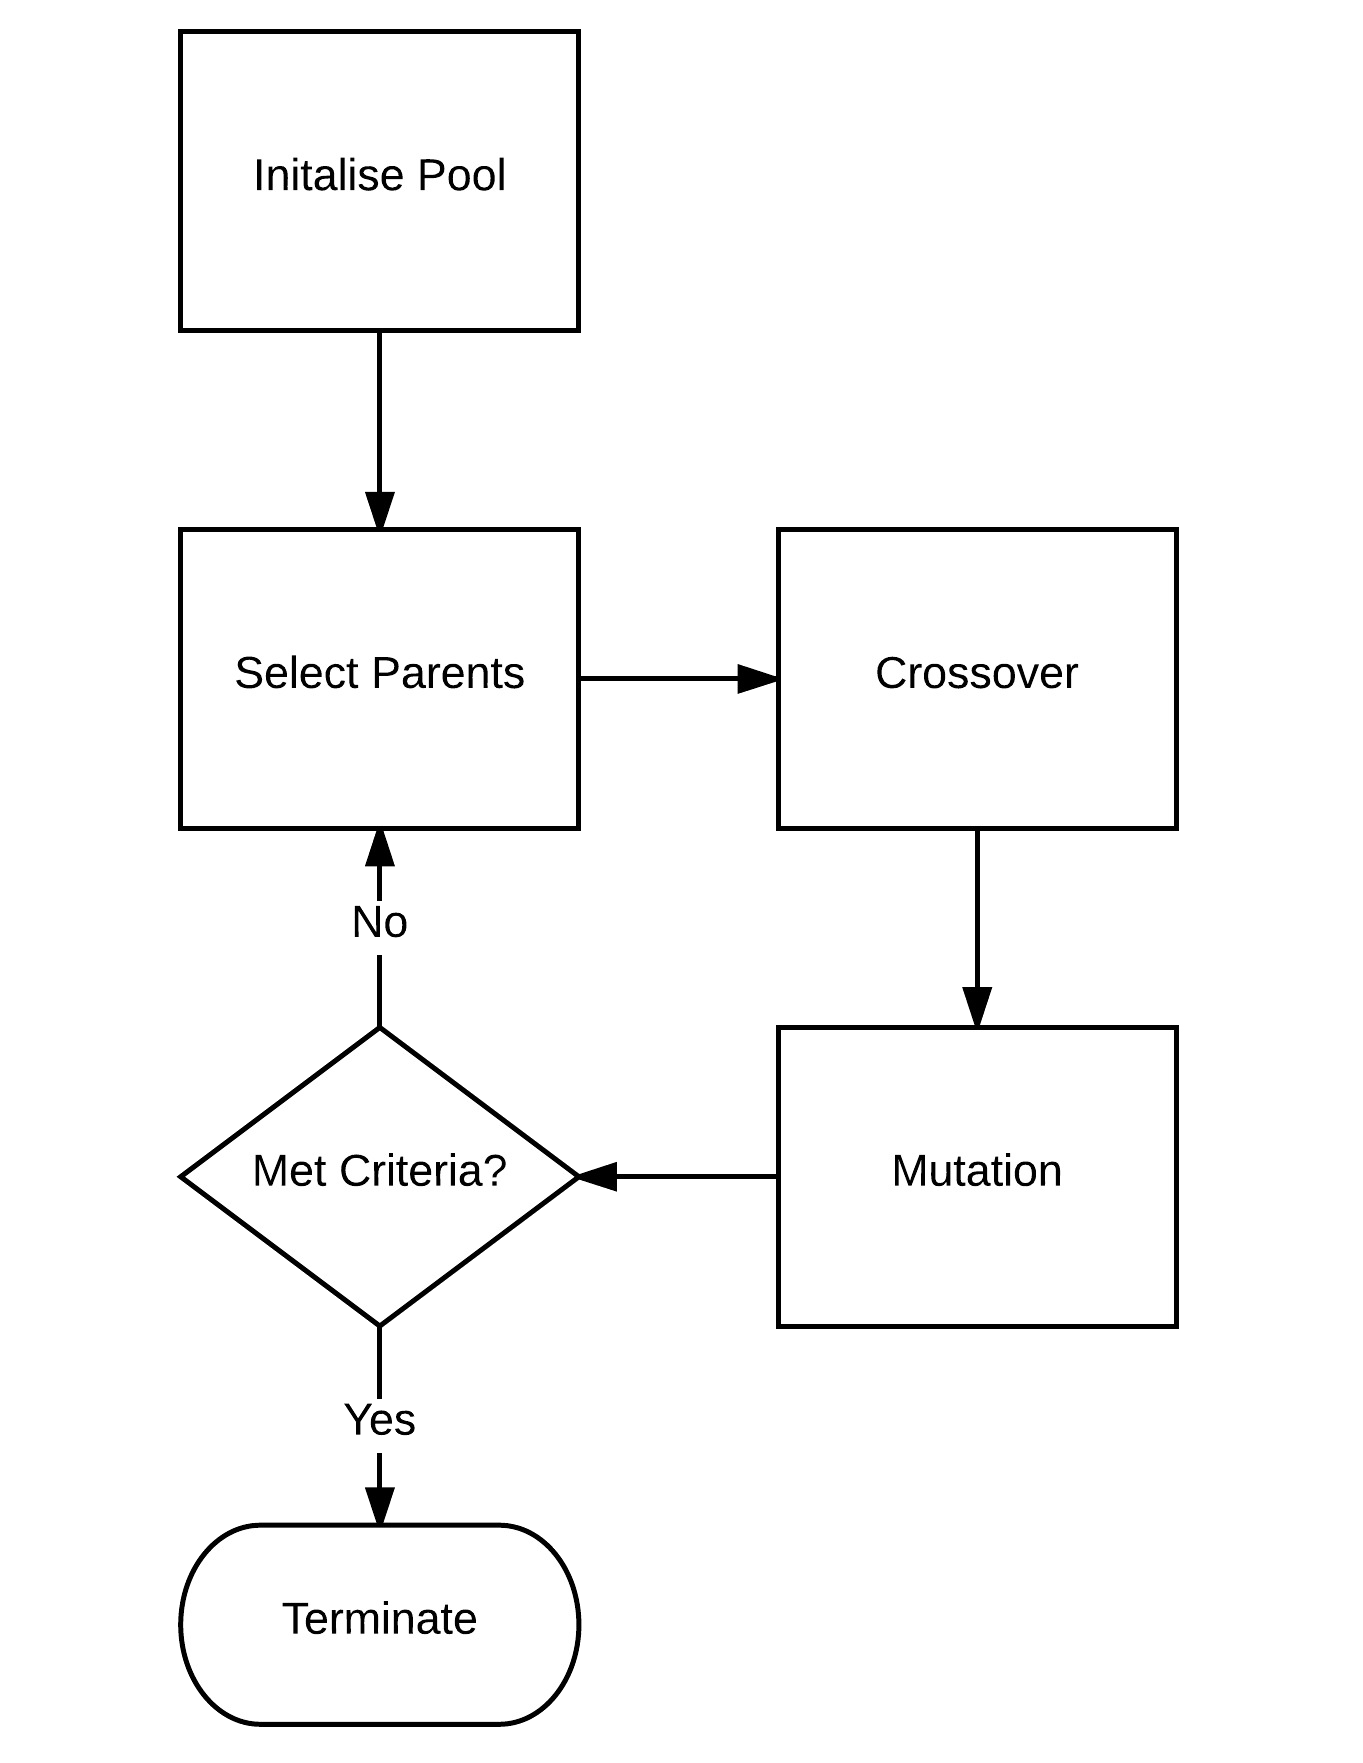
\includegraphics[width=0.5\textwidth]{GA_Structure}
	\caption{The basic structure of a Genetic Algorithm.}
	\label{struct}
\end{figure}
\noindent
A Genetic Algorithm is an algorithm that uses natural selection, or survival of the fittest, to find a solution to a problem. All Genetic Algorithms follow a similar, if not identical structure (figure \ref{struct}). However, the elements of this structure are highly customised for each specific application. Before going into detail about these elements, the concept of chromosomes and fitness must first be introduced.
\par
Chromosomes are one of the most important part of a GA, their only purpose is to store the potential solutions of the problem. How chromosomes store these solutions is up to the constructor of the GA, commonly however they are a single string that might represent a binary number, or possibly a list of the problems variables. Another important thing about chromosomes is their fitness. The fitness function of a GA describes how fit a particular problem is as a solution. How this fitness works, and how fitnesses are compared is again nearly entirely up to the constructor of the GA.


\section{Initialisation of the Pool}
\par
The first step in the execution of a Genetic algorithm is the generation of the pool. The pool is a collection of chromosomes that can be described as the "current generation". This pool is initialised by randomly generating chromosomes until the pool is filled, in the case of the research algorithm, this was done by shuffling the list of cities, thus eliminating the possibility of missing or having duplicate cities within the chromosome. The number of chromosomes in the pool is usually a fixed number, however adaptive pool sizing does exist (http://www.sciencedirect.com/science/article/pii/S2212671613000449) only fixed pool size was used in this research. 
\section{The Main Loop}
\par
This next section comprises the main body of the GA. Every time this loop is completed, a generation has passed. 
\subsection{Parent Selection}
\subsection{Crossover}
\subsubsection{Subbity Wubbity!}
\subsection{Mutation}
\section{Termination}
\section{The Research Framework}
\par
The Genetic Algorithm that was constructed for this research -----

